\section{Integrating Uncontrolled Loads\label{sec:uncontrolled}}
A monthly power bill is made up of several costs, two of which depend on the maximum energy consumed over 15 minutes. This 15-minute average power includes energy that is consumed by loads other than bus chargers, or "uncontrolled loads". In practice, data for uncontrolled loads is sampled and therefore discrete. The representations for how buses use power in Section \ref{sec:5_battery} are continuous, making their effects difficult to integrate with a discrete uncontrolled load. This section integrates these uncontrolled loads into the planning framework by converting the continuous start and end points, $c_{ij}$ and $s_{ij}$ from section \ref{sec:4_formulation}, to a vector $\mathbf{p}_{ij}$, where the $n^{\text{th}}$ element of $\mathbf{p}_{ij}$ represents the average power over the interval $t_{i-1}$ to $t_i$ from bus $i$ during route $j$. These route power vectors can be added together to form a discrete profile for the buses.
\par Let the day be divided into time segments, each of duration $\Delta T$. The first step is to determine the index of each segment that a bus begins charging, $k_{ij}^{\text{start}}$, and the index of the segement that a bus finishes charging, $k_{ij}^{\text{end}}$.  Each index can be computed as an integer multiple of $\Delta T$ that satisfies 
\begin{equation} \label{eqn:discrete1} \begin{aligned}
	\left ( k^{\text{start}}_{ij} - 1 \right ) \cdot\Delta T + r^{\text{start}}_{ij}&= c_{ij} \\
	\left (	k^{\text{end}}_{ij} - 1 \right ) \cdot\Delta T + r^{\text{end}}_{ij}&= s_{ij} \\
	k^{\text{start}}_{ij}, k^{\text{end}}_{ij} \in \mathbb{Z} \\
	0 < r^{\text{start}}_{ij}, r^{\text{end}}_{ij} < &\Delta T.
\end{aligned} \end{equation} 
Equation \eqref{eqn:discrete1} yields the discrete indices $k_{ij}^{\text{start}}$ and $k_{ij}^{\text{end}}$ along with corresponding remainder values $r_{ij}^{\text{start}}$ and $r_{ij}^{\text{end}}$ which will be used later in this section to calculate the average power for time segments in which buses only charge part of the time.  Equation (\ref{eqn:discrete1}) can be rewriten in standard form and zero padded such that
\begin{equation} \begin{aligned}
	\begin{bmatrix}\Delta T &  1 & -1 & 0        & 0 &  0\\ 
		       0        &  0 & 0  & \Delta T & 1 & -1\\
	\end{bmatrix} 
	\begin{bmatrix} k_{ij}^{\text{start}} \\
		        r_{ij}^{\text{start}} \\
			c_{ij}                \\
			k_{ij}^{\text{end}}   \\
			r_{ij}^{\text{end}}   \\
			s_{ij}
	\end{bmatrix} &= 
	\begin{bmatrix} 0 \\
	                0 \\
	\end{bmatrix} \ \forall i,j \\ 
	\tilde{A}_2\mathbf{y} &= \tilde{\mathbf{b}}_2.
\end{aligned} \end{equation}
and 
\begin{equation} \begin{aligned}
	\begin{bmatrix} 0 & -1 & 0 & 0 &  0 & 0\\
			0 &  1 & 0 & 0 &  0 & 0\\
		        0 &  0 & 0 & 0 & -1 & 0\\
			0 &  0 & 0 & 0 &  1 & 0\\
	\end{bmatrix} 
	\begin{bmatrix} k_{ij}^{\text{start}} \\
		        r_{ij}^{\text{start}} \\
			c_{ij}                \\
			k_{ij}^{\text{end}}   \\
			r_{ij}^{\text{end}}   \\
			s_{ij}
	\end{bmatrix} &\le 
	\begin{bmatrix}  0\\
			\Delta T \\
			0 \\
			\Delta T
	\end{bmatrix} \ \forall i,j \\ 
	A_6\mathbf{y} &\le \mathbf{b}_6.  
\end{aligned} \end{equation}
The next step is to use $k_{ij}^{\text{start}}$ and $k_{ij}^{\text{end}}$ to compute three sets of binary vectors, denoted $\mathbf{g}^{\text{start}}_{ij}$, $\mathbf{g}^{\text{on}}_{ij}$, and $\mathbf{g}^{\text{end}}_{ij}$, which act as selectors for indices which correspond to charge times. The values in $\mathbf{g}_{ij}^{\text{start}}$ and $\mathbf{g}_{ij}^{\text{end}}$ are equal to 1 during intervals that contain energy from the remainders $r_{ij}^{\text{start}}$ and $r_{ij}^{\text{end}}$. For example, the values for $\mathbf{g}_{ij}^{\text{start}}$ and $\mathbf{g}_{ij}^{\text{end}}$ from the scenario in Fig. \ref{fig:remainderB} would be 
\begin{equation}
	\mathbf{g}_{ij}^{\text{start}} = \begin{bmatrix}1 \\ 0 \\ 0 \\ 0 \end{bmatrix} \ \text{and} \ \mathbf{g}_{ij}^{\text{end}} = \begin{bmatrix}0 \\ 0 \\ 1 \\ 0 \end{bmatrix}.
\end{equation}
The values in $\mathbf{g}_{ij}^{\text{on}}$ will be equal to 1 for all time indices where buses charges the entire time. For example, the values in $g_{ij}^{\text{on}}$ that correspond to Fig. \ref{fig:remainderB} would be 
\begin{equation}
	\mathbf{g}_{ij}^{\text{on}} = \begin{bmatrix}0 \\ 1 \\ 0 \\ 0 \end{bmatrix}.
\end{equation}
\par Let $\mathbf{f}$ be a vector of one-based integer indices such that $f_w = w \ \forall w \in (1,\text{nPoint})$, where nPoint is the desired number of discrete samples. For example, if the day was discretized into $4$ periods, then $\mathbf{f}$ would be 
\begin{equation}
	\mathbf{f} = \begin{bmatrix}1 \\ 2 \\ 3 \\ 4 \end{bmatrix}.
\end{equation}
Defining the index as an element of $\mathbf{f}$ allows us to convert from the single indices $k_{ij}^{\text{start}}$ and $k_{ij}^{\text{end}}$ to the binary vectors $\mathbf{g}_{ij}^{\text{start}}$ and $\mathbf{g}_{ij}^{\text{end}}$ by letting 
\begin{equation}\label{eqn:idxStart}\begin{aligned}
	k^{\text{start}}_{ij}        &= \mathbf{f}^T\mathbf{g}^{\text{start}}_{ij} \\
	k^{\text{end}}_{ij}         &= \mathbf{f}^T\mathbf{g}^{\text{end}}_{ij}  \\ 
	1                            &= \mathbf{1}^T\mathbf{g}^{\text{start}}_{ij} \\
	1                            &= \mathbf{1}^T\mathbf{g}^{\text{end}}_{ij}  \\
	\mathbf{g}^{\text{start}}_{ij}  &\in \{0,1\}^{\text{nPoint}}                \\
	\mathbf{g}^{\text{end}}_{ij} &\in \{0,1\}^{\text{nPoint}},
\end{aligned} \end{equation}

which can be expressed in standard form and zero padded to form a set of linear constraints.
\begin{equation} \label{eqn:idxStart2}\begin{aligned}
	\begin{bmatrix} 0 & \mathbf{0}^T & -1 & \mathbf{f}^T \\
		        0 & \mathbf{1}^T &  0 & 0            \\
		       -1 & \mathbf{f}^T & 0 & \mathbf{0}^T  \\
		        0 & 0            & 0 & \mathbf{1}^T 
	\end{bmatrix} 
	\begin{bmatrix} k_{ij}^{\text{start}}       \\
		        \mathbf{g}_{ij}^{\text{start}} \\ 
			k_{ij}^{\text{end}}        \\ 
			\mathbf{g}_{ij}^{\text{end}} 
	\end{bmatrix} &= 
	\begin{bmatrix} 0 \\ 
			1 \\
	                0 \\
			1
	\end{bmatrix} \ \forall i,j \\
	\tilde{A}_3\mathbf{y} &= \tilde{\mathbf{b}}_3.
\end{aligned} \end{equation}
\begin{figure}
\centering
	\subfloat[Continuous Charging Segment\label{fig:remainderA}]{
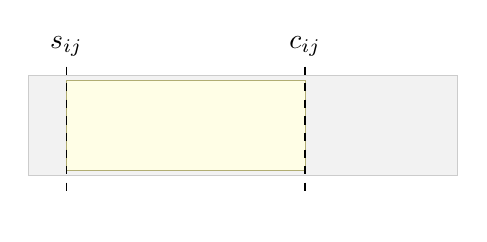
\begin{tikzpicture}
	\node[rectangle, draw=gray!40, fill=gray!10, minimum width=0.45\textwidth, minimum height=0.5in](bus) at (0,0){};	
	\node[rectangle, draw=yellow!50!black!70, fill=yellow!10, minimum width=0.25\textwidth, minimum height=0.45in](charge) at (-0.06\textwidth,0){};
	\node(topLeft) at (-0.185\textwidth,1){$s_{ij}$};
	\node(btmLeft) at (-0.185\textwidth,-1){};
	\draw[dashed, line width=0.5pt](topLeft) -- (btmLeft);
	\node(topRight) at (0.065\textwidth,1){$c_{ij}$};
	\node(btmRight) at (0.065\textwidth,-1){};
	\draw[dashed, line width=0.5pt](topRight) -- (btmRight);
\end{tikzpicture}
}%

	\subfloat[Discrete Charging Segments\label{fig:remainderB}]{
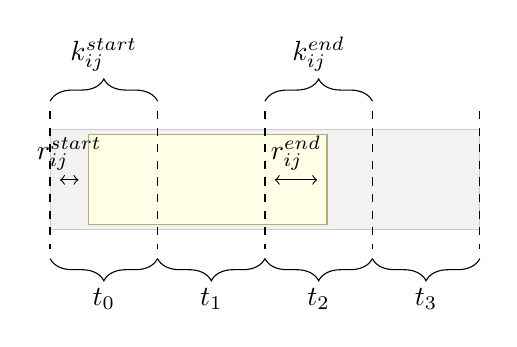
\begin{tikzpicture}
	\node[rectangle, draw=gray!40, fill=gray!10, minimum width=0.45\textwidth, minimum height=0.5in](bus) at (0,0){};	
	\node[rectangle, draw=yellow!50!black!70, fill=yellow!10, minimum width=0.25\textwidth, minimum height=0.45in](charge) at (-0.06\textwidth,0){};
	\node(top0) at (-0.225\textwidth,1){};
	\node(top1) at (-0.1125\textwidth,1){};
	\node(top2) at (0\textwidth,1){};
	\node(top3) at (0.1125\textwidth,1){};
	\node(top4) at (0.225\textwidth,1){};

	\node(btm0) at (-0.225\textwidth ,-1){};
	\node(btm1) at (-0.1125\textwidth,-1){};
	\node(btm2) at (0\textwidth      ,-1){};
	\node(btm3) at (0.1125\textwidth ,-1){};
	\node(btm4) at (0.225\textwidth  ,-1){}; 
	
	\draw[dashed, line width=0.5pt](top0) -- (btm0);
	\draw[dashed, line width=0.5pt](top1) -- (btm1);
	\draw[dashed, line width=0.5pt](top2) -- (btm2);
	\draw[dashed, line width=0.5pt](top3) -- (btm3);
	\draw[dashed, line width=0.5pt](top4) -- (btm4);

	\draw[decorate, decoration={brace, amplitude=8, mirror}](btm0.center) -- (btm1.center) node [midway, below=0.1in]{$t_0$};
	\draw[decorate, decoration={brace, amplitude=8, mirror}](btm1.center) -- (btm2.center) node [midway, below=0.1in]{$t_1$};
	\draw[decorate, decoration={brace, amplitude=8, mirror}](btm2.center) -- (btm3.center) node [midway, below=0.1in]{$t_2$};
	\draw[decorate, decoration={brace, amplitude=8, mirror}](btm3.center) -- (btm4.center) node [midway, below=0.1in]{$t_3$};

	\draw[decorate, decoration={brace, amplitude=8}](top0.center) -- (top1.center) node [midway, above=0.1in]{$k_{ij}^{\text{start}}$};
	\draw[decorate, decoration={brace, amplitude=8}](top2.center) -- (top3.center) node [midway, above=0.1in]{$k_{ij}^{\text{end}}$};


	\node(s0) at (-0.225\textwidth,0){};
	\node(s1) at (-0.185\textwidth,0){};
	\draw[<->](s0) -- node[above]{$r_{ij}^{\text{start}}$} ++ (s1); 
	
	\node(c0) at (0.065\textwidth,0){};
        \node(c1) at (0.0\textwidth,0){};
	\draw[<->](c0) -- node[above]{$r_{ij}^{\text{end}}$} ++ (c1); 
\end{tikzpicture} 
}
	\caption{Discretization of continuous charging intervals}
\end{figure}

 The values of $\mathbf{g}_{ij}^{\text{on}}$ can be computed by first noticing that indices that correspond to complete charge intervals must remain between $k_{ij}^{\text{start}}$ and $k_{ij}^{\text{end}}$, implying that 
\begin{equation}\label{eqn:gOnCases}\begin{aligned}
	\begin{rcases}
		\begin{array}{ll}
			g_w f_w \le k^{\text{end}} - 1  \\
			g_w f_w \ge k^{\text{start}} + 1\\ 
		\end{array} & g_w = 1 \\
	\end{rcases},
\end{aligned} \end{equation}
which can be expressed as a set of linear constraints such that
\begin{equation} \label{eqn:gOnBigM}\begin{aligned}
	g_w\cdot f_w &\le k^{\text{end}}_{ij} + M(1 - g_w) - 1 \\
	g_w\cdot f_w &\ge k^{\text{start}}_{ij} - M(1 - g_w) + 1 \\ 
\end{aligned} \end{equation}
where $M$ is $2\cdot\text{nPoint}$. The constraints in \eqref{eqn:gOnBigM} do not require that all values between $k_{ij}^{\text{start}}$ and $k_{ij}^{\text{end}}$ be set to one however, only that if a value is equal to one, that it must be between $k_{ij}^{\text{start}}$ and $k_{ij}^{\text{end}}$. For all values between  $k_{ij}^{\text{start}}$ and $k_{ij}^{\text{end}}$ to be $1$, the sum of $\mathbf{g}_{ij}^{\text{on}}$ must be equal to the difference between $k_{ij}^{\text{end}}$ and $k_{ij}^{\text{start}}$ such that 
\begin{equation} \label{eqn:gOnSemiFinal}\begin{aligned}
	g_w\cdot f_w &\le k^{\text{end}}_{ij} + M(1 - g_w) - 1 \\
	g_w\cdot f_w &\ge k^{\text{start}}_{ij} - M(1 - g_w) + 1 \\ 
	\mathbf{1}^T\mathbf{g}_{ij}^{\text{on}} &= k_{ij}^{\text{end}} - k_{ij}^{\text{start}} - 1.\\
\end{aligned} \end{equation}
The constraints in \eqref{eqn:gOnSemiFinal} work well for a general use case, however when $k_{ij}^{\text{end}}$ is equal to $k_{ij}^{\text{start}}$, the last constraint in equation (\ref{eqn:gOnSemiFinal}) becomes
\begin{equation}
	\mathbf{1}^T\mathbf{g}_{ij}^{\text{on}} = -1
\end{equation}
which leads to an empty feasible set because all the elements of $\mathbf{g}_{ij}^{\text{on}}$ are binary. Let $k_{ij}^{\text{eq}}$ be a binary variable which is equal to $0$ when $k_{ij}^{\text{end}}$ is not equal to $k_{ij}^{\text{start}}$. Equation \eqref{eqn:gOnSemiFinal} can be modified to incorporate $k_{ij}^{\text{eq}}$ to switch between the cases where $k_{ij}^{\text{end}}$ is equal, and not equal to $k_{ij}^{\text{start}}$ by letting 
\begin{equation} \label{eqn:gOnFinal}\begin{aligned}
	g_w\cdot f_w &\le k^{\text{end}}_{ij} + M(1 - g_w) - 1 \\
	g_w\cdot f_w &\ge k^{\text{start}}_{ij} - M(1 - g_w) + 1 \\ 
	\mathbf{1}^T\mathbf{g}_{ij}^{\text{on}} &= k_{ij}^{\text{end}} - k_{ij}^{\text{start}} - k_{ij}^{\text{eq}}.\\
\end{aligned} \end{equation} 
 and constraining $k_{ij}^{\text{eq}}$ such that 
\begin{equation}\label{eqn:kEq}\begin{aligned}
	k_{ij}^{\text{end}} - k_{ij}^{\text{start}} - M k_{ij}^{\text{eq}} \le 0 \\
	-k_{ij}^{\text{end}} + k_{ij}^{\text{start}} + M k_{ij}^{\text{eq}} \le M .
\end{aligned}\end{equation}
The constraints from \eqref{eqn:gOnFinal} and \eqref{eqn:kEq} can be expressed in standard form as 
\begin{equation} \label{eqn:gOnFinalStd}\begin{aligned}
	\mathbf{1}^T\mathbf{g}_{ij}^{\text{on}} - k_{ij}^{\text{end}} + k_{ij}^{\text{start}} + k_{ij}^{\text{eq}} &=  0 \\
	k_{ij}^{\text{end}} - k_{ij}^{\text{start}} - M k_{ij}^{\text{eq}} &\le 0 \\
	-k_{ij}^{\text{end}} + k_{ij}^{\text{start}} + M k_{ij}^{\text{eq}} &\le M \\
	g_w\left (f_w + M \right) - k_{ij}^{\text{end}} &\le M - 1 \\
	g_w\left (M - f_w\right) + k_{ij}^{\text{start}} &\le M - 1.
\end{aligned}\end{equation}
The inequality constriants from equation (\ref{eqn:gOnFinalStd}) imply that
\begin{equation} \label{eqn:gOnFinalPart1}\begin{aligned}
	\begin{bmatrix}f_w + M & -1 & 0\\
		       M - f_w & 0 & 1 
	\end{bmatrix} 
	\begin{bmatrix}g_w                 \\
		       k_{ij}^{\text{end}} \\ 
		       k_{ij}^{\text{start}}
	\end{bmatrix} \le
	\begin{bmatrix} M - 1 \\
	                M - 1 
	\end{bmatrix} \forall g_w \in \mathbf{g}_{ij}^{\text{on}}
\end{aligned}\end{equation} 
and that
\begin{equation} \label{eqn:kEqStd}\begin{aligned}
	\begin{bmatrix}1 & -1 & -M \\
		       -1 & 1 & M  \\
		       \end{bmatrix} \begin{bmatrix}k_{ij}^{\text{end}} \\ k_{ij}^{\text{start}} \\ k_{ij}^{\text{eq}} \end{bmatrix} \le \begin{bmatrix} 0 \\ M\end{bmatrix} \ \forall i,j,
\end{aligned} \end{equation}
which can be concatenated for all $i,j$ and zero padded to form a joint matrix, satisfying 
\begin{equation}
	A_7\mathbf{y} \le \mathbf{b}_7.
\end{equation}
Similarly, the equality constraint from equation (\ref{eqn:gOnFinalStd}) can also be concatenated and zero padded such that
\begin{equation} \begin{aligned}
	\mathbf{1}^T\mathbf{g}_{ij}^{\text{on}} - k_{ij}^{\text{end}} + k_{ij}^{\text{start}} + k_{ij}^{\text{eq}} &= 0 \ \forall i,j\\
	\begin{bmatrix}\mathbf{1}^T & - 1 & 1 & -1\end{bmatrix} \begin{bmatrix}\mathbf{g}_{ij}^{\text{on}} \\ k_{ij}^{\text{end}} \\ k_{ij}^{\text{start}} \\ k_{ij}^{\text{eq}} \end{bmatrix} &= 0 \\
		\tilde{A}_4\mathbf{y} &= \tilde{\mathbf{b}}_4.
\end{aligned} \end{equation}
	\par The next step is to define the average power during intervals that only charge for part of the time.  These intervals correspond to the remainder values $r_{ij}^{\text{start}}$ and $r_{ij}^{\text{end}}$ and, as with previous constraints, maintain different behavior when $k_{ij}^{\text{eq}} = 0$ and $k_{ij}^{\text{eq}} = 1$. The average power that corresponds to $r_{ij}^{\text{start}}$ and $r_{ij}^{\text{end}}$ can be computed as 
\begin{equation}\label{eqn:avgPower1}\begin{aligned}
	\begin{rcases}
	\begin{array}{l} \begin{aligned}
		p^{\text{start}}_{ij} &= \frac{p\cdot (\Delta T - r^{\text{start}}_{ij})}{\Delta T}\\ 
		p^{\text{end}}_{ij} &= \frac{p\cdot r^{\text{end}}_{ij}}{\Delta T}.\\
	\end{aligned} \end{array} & k_{ij}^{\text{eq}} = 1 \\[8pt] 
	\begin{array}{l} \begin{aligned}
		p_{ij}^{\text{start}} &= \frac{p\cdot \left ( r_{ij}^{\text{end}} - r_{ij}^{\text{start}} \right )}{\Delta T} \\
		p_{ij}^{\text{end}} &= 0 \\
	\end{aligned} \end{array} & k_{ij}^{\text{eq}} = 0 \\
	\end{rcases}.
\end{aligned}\end{equation}
Equation \eqref{eqn:avgPower1} can also be expressed as a set of linear inequality constraints such that
\begin{equation} \begin{aligned}
	p_{ij}^{\text{start}} &\le p - \frac{p}{\Delta T}r_{ij}^{\text{start}} + M\left ( 1 - k_{ij}^{\text{eq}} \right ) \\
	p_{ij}^{\text{start}} &\ge p - \frac{p}{\Delta T}r_{ij}^{\text{start}} - M\left ( 1 - k_{ij}^{\text{eq}} \right ) \\ 
	p_{ij}^{\text{start}} &\le \frac{p}{\Delta T}r_{ij}^{\text{end}} - \frac{p}{\Delta T}r_{ij}^{\text{start}} + Mk_{ij}^{\text{eq}}\\
	p_{ij}^{\text{start}} &\ge \frac{p}{\Delta T}r_{ij}^{\text{end}} - \frac{p}{\Delta T}r_{ij}^{\text{start}} - Mk_{ij}^{\text{eq}}\\ 
	p_{ij}^{\text{end}}   &\le \frac{p}{\Delta T}r_{ij}^{\text{end}} + M\left ( 1 - k_{ij}^{\text{eq}} \right )\\
	p_{ij}^{\text{end}}   &\ge \frac{p}{\Delta T}r_{ij}^{\text{end}} - M\left ( 1 - k_{ij}^{\text{eq}} \right )\\
	p_{ij}^{\text{end}}   &\le Mk_{ij}^{\text{eq}}\\
	p_{ij}^{\text{end}}   &\ge - Mk_{ij}^{\text{eq}},\\
\end{aligned} \end{equation}
where $M$ is the battery capacity, and can be expressed in standard form as
\begin{equation} \begin{aligned}
	 p_{ij}^{\text{start}} + \frac{p}{\Delta T} r_{ij}^{\text{start}} + Mk_{ij}^{\text{eq}} &\le M + p \\
	-p_{ij}^{\text{start}} - \frac{p}{\Delta T} r_{ij}^{\text{start}} + Mk_{ij}^{\text{eq}} &\le M - p \\
	 p_{ij}^{\text{start}} - \frac{p}{\Delta T} r_{ij}^{\text{end}}  + \frac{p}{\Delta T}r_{ij}^{\text{start}} - Mk_{ij}^{\text{eq}} &\le 0\\
	-p_{ij}^{\text{start}} + \frac{p}{\Delta T} r_{ij}^{\text{end}}  - \frac{p}{\Delta T}r_{ij}^{\text{start}} - Mk_{ij}^{\text{eq}} &\le 0\\
	 p_{ij}^{\text{end}}   - \frac{p}{\Delta T} r_{ij}^{\text{end}} + Mk_{ij}^{\text{eq}} &\le M \\
	-p_{ij}^{\text{end}}   + \frac{p}{\Delta T} r_{ij}^{\text{end}} + Mk_{ij}^{\text{eq}} &\le M \\
	 p_{ij}^{\text{end}}   - Mk_{ij}^{\text{eq}} &\le 0\\
	-p_{ij}^{\text{end}}   - Mk_{ij}^{\text{eq}}&\le 0 \\
\end{aligned} \end{equation}
and by using matrix multiplication such that
\begin{equation}\begin{aligned}
	\begin{bmatrix} 
		 1 &  0 &  \frac{p}{\Delta T} &  0                  &  M\\
		-1 &  0 & -\frac{p}{\Delta T} &  0                  &  M\\
		 1 &  0 &  \frac{p}{\Delta T} & -\frac{p}{\Delta T} & -M\\ 
		-1 &  0 & -\frac{p}{\Delta T} &  \frac{p}{\Delta T} & -M\\
		 0 &  1 & 0                   & -\frac{p}{\Delta T} &  M\\
		 0 & -1 & 0                   &  \frac{p}{\Delta T} &  M\\
		 0 &  1 & 0                   &  0                  & -M\\
		 0 & -1 & 0                   &  0                  & -M\\
	\end{bmatrix} 
	\begin{bmatrix}
		p_{ij}^{\text{start}} \\
                p_{ij}^{\text{end}} \\
                r_{ij}^{\text{start}} \\
                r_{ij}^{\text{end}} \\
                k_{ij}^{\text{eq}}
	\end{bmatrix} &\le 
	\begin{bmatrix}
		M + p \\
		M - p \\
		0 \\
		0 \\
		M \\
		M \\
		0 \\
		0 \\
	\end{bmatrix} \ \forall i,j \\
	A_8 &\le \mathbf{b}_8
\end{aligned}\end{equation} 
where $p_{ij}^{\text{start}}$, $p_{ij}^{\text{end}}$, and $p$ represent the average power that corresponds to $r_{ij}^{\text{start}}$, $r_{ij}^{\text{end}}$, and full charging intervals respectively. The total average power use is calculated as 
\begin{align}\label{eqn:totalPower}
	\mathbf{p}_{\text{total}} = \bar{\mathbf{p}}_{\text{load}} + \sum_{ij} \mathbf{g}^{\text{start}}_{ij}\cdot p^{\text{start}}_{ij} + \mathbf{g}^{\text{on}}_{ij}\cdot p + \mathbf{g}^{\text{end}}_{ij}\cdot p^{\text{end}}_{ij}
\end{align}
where $\bar{\mathbf{p}}_{\text{load}}$ is the average power of the uncontrolled loads.
\par Note, however that \eqref{eqn:totalPower} contains the bilinear terms $\mathbf{g}_{ij}^{\text{start}}\cdot p_{ij}^{\text{start}}$ and $\mathbf{g}_{ij}^{\text{end}}\cdot p_{ij}^{\text{end}}$. The expression $\mathbf{g}_{ij}^{\text{start}}\cdot p_{ij}^{\text{start}}$ from \eqref{eqn:totalPower} can be thought of as a vector, $\mathbf{p}_{ij}^{\text{start}}$ which contains values for $p_{ij}^{\text{start}}$ whenever $g_{ij}^{\text{start}}$ is not equal to $0$ such that 
\begin{equation} \label{eqn:bilinear1}\begin{aligned}
	\begin{rcases}
		p_w = p^{\text{start}} & g_w = 1 \\
		p_w = 0                & g_w = 0 \\
	\end{rcases} \forall p_w \in \mathbf{p}_{ij}^{\text{start}},
\end{aligned} \end{equation}
which can be rewritten as a set of linear inequality constraints such that
\begin{equation} \label{eqn:onPower}\begin{aligned}
	p_w &\ge p^{\text{start}}_{ij} - M(1 - g_w) \forall p_w \in \mathbf{p}_{ij}^{\text{start}}\\
	p_w &\le p^{\text{start}}_{ij} + M(1 - g_w) \forall p_w \in \mathbf{p}_{ij}^{\text{start}}\\
	p_w &\ge -Mg_w \forall p_w \in \mathbf{p}_{ij}^{\text{start}}\\
	p_w &\le  Mg_w \forall p_w \in \mathbf{p}_{ij}^{\text{start}}
\end{aligned} \end{equation}
The same approach can be taken to replace $\mathbf{g}_{ij}^{\text{end}}\cdot p_{ij}^{\text{end}}$ with the vector $\mathbf{p}_{ij}^{\text{end}}$ by letting
\begin{equation} \label{eqn:offPower} \begin{aligned}
	p_w &\ge p^{\text{end}}_{ij} - M(1 - g_w) \ \forall p_w \in \mathbf{p}_{ij}^{\text{end}}\\
	p_w &\le p^{\text{end}}_{ij} + M(1 - g_w) \ \forall p_w \in \mathbf{p}_{ij}^{\text{end}}\\
	p_w &\ge -Mg_w \ \forall p_w \in \mathbf{p}_{ij}^{\text{end}}\\
	p_w &\le Mg_w \  \forall p_w \in \mathbf{p}_{ij}^{\text{end}},
\end{aligned} \end{equation} 
which can be written in standard form, stacked to accomodate the constraints for all $i,j$, and zero padded in the usual fashion as
\begin{equation}\begin{aligned} 
	\begin{bmatrix}
		-1 & 1 & M \\
		1  & -1 & M \\
		-1 & 0 & -M \\
		1 & 0 & -M 
	\end{bmatrix}
	\begin{bmatrix} 
		p_w                     \\
	        p_{ij}^{\text{start}} \\
		g_w
	\end{bmatrix}  &\le
	\begin{bmatrix}
		M \\
		M \\
		0 \\
		0
	\end{bmatrix} \forall p_w \in \mathbf{p}_{ij}^{\text{start}}\\ 
	A_9 &\le \mathbf{b}_9.
\end{aligned}\end{equation}
	Equation \eqref{eqn:offPower} can be expressed in standard form, stacked for all $i,j$, and zero padded in a similar fashion such that 
\begin{equation}\begin{aligned} 
	\begin{bmatrix}
		-1 & 1 & M  \\
		1  & -1 & M \\
		-1 & 0 & -M \\
		1 & 0 & -M 
	\end{bmatrix}	
	\begin{bmatrix} p_w                      \\
		        p_{ij}^{\text{end}} \\
			g_w
	\end{bmatrix} &\le
	\begin{bmatrix} M \\
	                M \\
	                0 \\
	                0
	\end{bmatrix} \ \forall p_w \in \mathbf{p}_{ij}^{\text{end}} \\
	A_{10}\mathbf{y} & \le \mathbf{b}_{10}.
\end{aligned}\end{equation} 
An expression for the total power used can then be expressed as
\begin{equation}
	\begin{aligned}
		\mathbf{p}^{\text{total}} = \mathbf{p}^{\text{load}} + \sum_{ij} \mathbf{p}^{\text{start}}_{ij} + \mathbf{p}^{\text{end}}_{ij} + \mathbf{g}^{\text{on}}_{ij}\cdot p
	\end{aligned}
\end{equation}
and in standard form as
\begin{equation} \begin{aligned}
	\begin{bmatrix}
		1 & -1^{\text{start}} & -1^{\text{end}} & -1^{\text{on}}\cdot p  
	\end{bmatrix}
	\begin{bmatrix}
		\mathbf{p}_{w}^{\text{total}} \\
	        \mathbf{p}_{w}^{\text{start}} \\
	        \mathbf{p}_{w}^{\text{end}}   \\
	        \mathbf{g}_{w}^{\text{on}}    \\
	\end{bmatrix} &= \mathbf{p}_{w}^{\text{load}}  \\
	\tilde{A}_4\mathbf{y} &= \tilde{\mathbf{b}}_4
\end{aligned} \end{equation}

